
%(BEGIN_QUESTION)
% Copyright 2015, Tony R. Kuphaldt, released under the Creative Commons Attribution License (v 1.0)
% This means you may do almost anything with this work of mine, so long as you give me proper credit

Sketch connecting wires to allow this data acquisition (DAQ) module to indicate temperature at input channel {\tt IN 3} from the thermocouple's voltage signal (i.e. higher temperature results in a stronger positive reading at the DAQ).  Feel free to add any additional components you deem necessary to this circuit, as you will need to account for the DAQ's bias current requirements!

\vskip 50pt

$$\includegraphics[width=15.5cm]{i04699x01.eps}$$

\underbar{file i04699}
%(END_QUESTION)





%(BEGIN_ANSWER)

Any solution providing a path for input bias currents to get to the AI Gnd terminal is acceptable.  This may take the form of bias resistors, or simply connecting one of the thermocouple leads to AI Gnd (either through a resistor to ground or directly to ground):

$$\includegraphics[width=15.5cm]{i04699x02.eps}$$

%(END_ANSWER)





%(BEGIN_NOTES)

{\bf This question is intended for exams only and not worksheets!}.

%(END_NOTES)

